\section{Einleitung}
In der vorliegenden Arbeit bereiten wir die Publikation \textit{Orthogonal Projections of Symmetric Polyhedra} von N. Hungerbühler und Y. Zhang \cite{hungerbuehler_symmetric_polyhedra} für ein breiteres Publikum auf. Die Zielgruppe umfasst unter anderem interessierte Schülerinnen und Schüler, Studierende sowie Lehrpersonen. Diese Arbeit führt die notwendige Theorie ein, um die zentralen Ideen und Berechnungen der Originalpublikation nachzuvollziehen. Im ersten Kapitel werden die grundlegenden Begriffe und Konzepte etabliert, während Kapitel \ref{sec:orthogonalprojektionen} den Beweis der Hauptaussage behandelt. Wir beginnen mit einem Einführungsbeispiel, das die Erkenntnisse der Publikation motivieren und veranschaulichen soll. Darauf folgt eine Einführung bzw. Repetition zu regulären Polyedern, Symmetriegruppen und Orthogonalprojektionen. Mit diesem theoretischen Fundament sind wir anschließend in der Lage, die mathematischen Aussagen in Kapitel \ref{sec:orthogonalprojektionen} fundiert zu beweisen.

 \subsection{Einführungsbeispiel}
Das zentrale Thema dieses Abschnitts sind Orthogonalprojektionen regulärer Polyeder auf Ebenen. Als Einstieg betrachten wir die Projektion eines Würfels auf eine Ebene im Raum. Der Würfel, auch \textbf{reguläres Hexaeder} genannt, siehe Abb. \ref{fig:einheitswürfel}, besitzt zahlreiche interessante Merkmale. Dazu gehören insbesondere seine Symmetrieeigenschaften, welche in Abschnitt \ref{sec:symmetrieeigenschaftwürfel} detailliert analysiert werden. Im Rahmen dieses Einführungsbeispiels fokussieren wir uns jedoch primär auf eine spezifische Eigenschaft der Kantenlängen der Orthogonalprojektion.

\begin{figure}[htp]
    \centering
    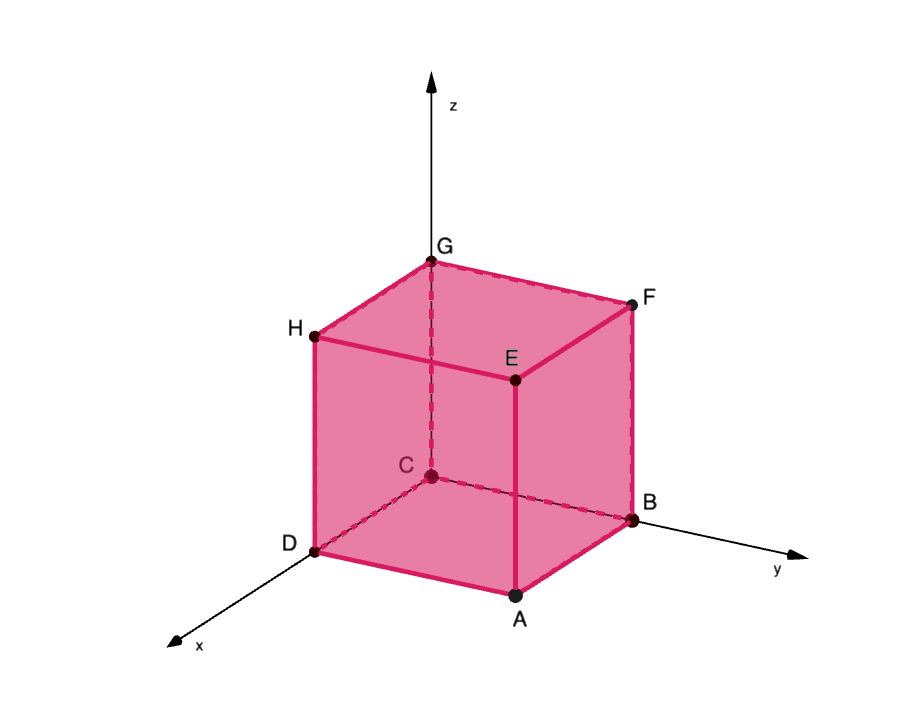
\includegraphics[width=0.7\textwidth, keepaspectratio]{images/einleitung/wuerfel_ortho_projektionen.png} 
    \caption{Regulärer Hexaeder $W$ mit Eckpunkten $A, B, \dots, H$.}
    \label{fig:einheitswürfel}
\end{figure}

Wir untersuchen, ob es eine invariante Eigenschaft in Bezug auf die projizierten Kantenlängen gibt. Eine Hypothese könnte lauten, dass die Summe der Längen aller projizierten Kanten eines Würfels bei einer Orthogonalprojektion unabhängig von der Lage der Projektionsebene ist. Um die Plausibilität dieser Hypothese zu prüfen, betrachten wir zunächst die Projektionen der Würfelkanten auf zwei verschiedene Ebenen. Sollte die Eigenschaft bereits für diese zwei Fälle nicht gelten, liesse sich die Hypothese direkt widerlegen. Das Nachvollziehen von Hypothesen an konkreten Instanzen ist zudem oftmals hilfreich, um ein besseres Verständnis aufzubauen und möglicherweise eine bessere Hypothese zu finden. Dieser Untersuchung gehen wir in Beispiel \ref{ex:wuerfelprojektionen} nach.



\begin{example}[Orthogonalprojektionen der Kanten eines Würfels auf eine Ebene] \label{ex:wuerfelprojektionen} 
Seien $E_1, E_2 \subset \mathbb{R}^3$ zwei Ebenen gegeben durch 

\begin{align}
    E_1:\ &x+y+z = 0,  \label{eq:ebene1}\\
    E_2:\ &x-y = 0 . \label{eq:ebene2}
\end{align}

 Sei $K_W$ die Menge der Kanten eines Würfels $W$, welcher in Abbildung \ref{fig:einheitswürfel} dargestellt ist. Wir wollen überprüfen, ob die Summe der Kantenlängen von einer Orthogonalprojektion auf diese beiden Ebenen identisch ist. Diese Behauptung kann wie folgt formuliert werden
\begin{align} \label{eq:hypothese1}
    \sum_{k \in K_W} \|\Pi_{E_1}(\vec{v}_k)\| = \sum_{k \in K_W} \|\Pi_{E_2}(\vec{v}_{k})\|,
\end{align}

wo $\Pi_{E_i}: \mathbb{R}^3 \rightarrow E_i$ die Orthogonalprojektion auf die Ebene $E_i \subset \mathbb{R}^3$ ist und $\vec{v}_k$ der zur Kante $k$ gehörende Richtungsvektor. Um diese Behauptung zu überprüfen, berechnen wir explizit die projizierten Kantenlängen eines regulären Hexaeders mit Kantenlänge $1$ und addieren diese auf. Diese Normierung vereinfacht die Rechnung, ohne die Allgemeingültigkeit einzuschränken, da die Ergebnisse für eine beliebige Kantenlänge $a$ lediglich um den Faktor $a$ skaliert würden. Die Ebene $E_1$, auf die wir projizieren, ist gegeben durch die Gleichung \eqref{eq:ebene1} mit dem Einheitsnormalenvektor 
\begin{align}
    \vec{n}_{E_1}  = \frac{1}{\sqrt{3}}\begin{pmatrix} 1 \\ 1 \\ 1 \end{pmatrix} .\nonumber
\end{align}

    \begin{figure}[htp]
    \centering
    \includegraphics[width=10cm]{images/einleitung/WürfelE1.png}
    \caption{Projektion der Kanten des Würfels auf die Ebene $E_1$ mit Normalenvektor $\vec{n}_{E_1}$.}
    \label{fig:würfelE1}
    \end{figure}

Bevor wir die Orthogonalprojektionen explizit berechnen, halten wir folgende Beobachtungen fest (siehe Abbildung \ref{fig:beobachtungenOrthogonalprojektionWurfel}):
\begin{itemize}
    \item Die Translation einer Strecke verändert die Länge ihrer Orthogonalprojektion auf eine Ebene nicht.
    \item Infolgedessen können wir jede Kante des Würfels als einen Vektor betrachten, indem wir ihren Fusspunkt in den Ursprung verschieben. 
\end{itemize}

    \begin{figure}[htp]
        \centering
        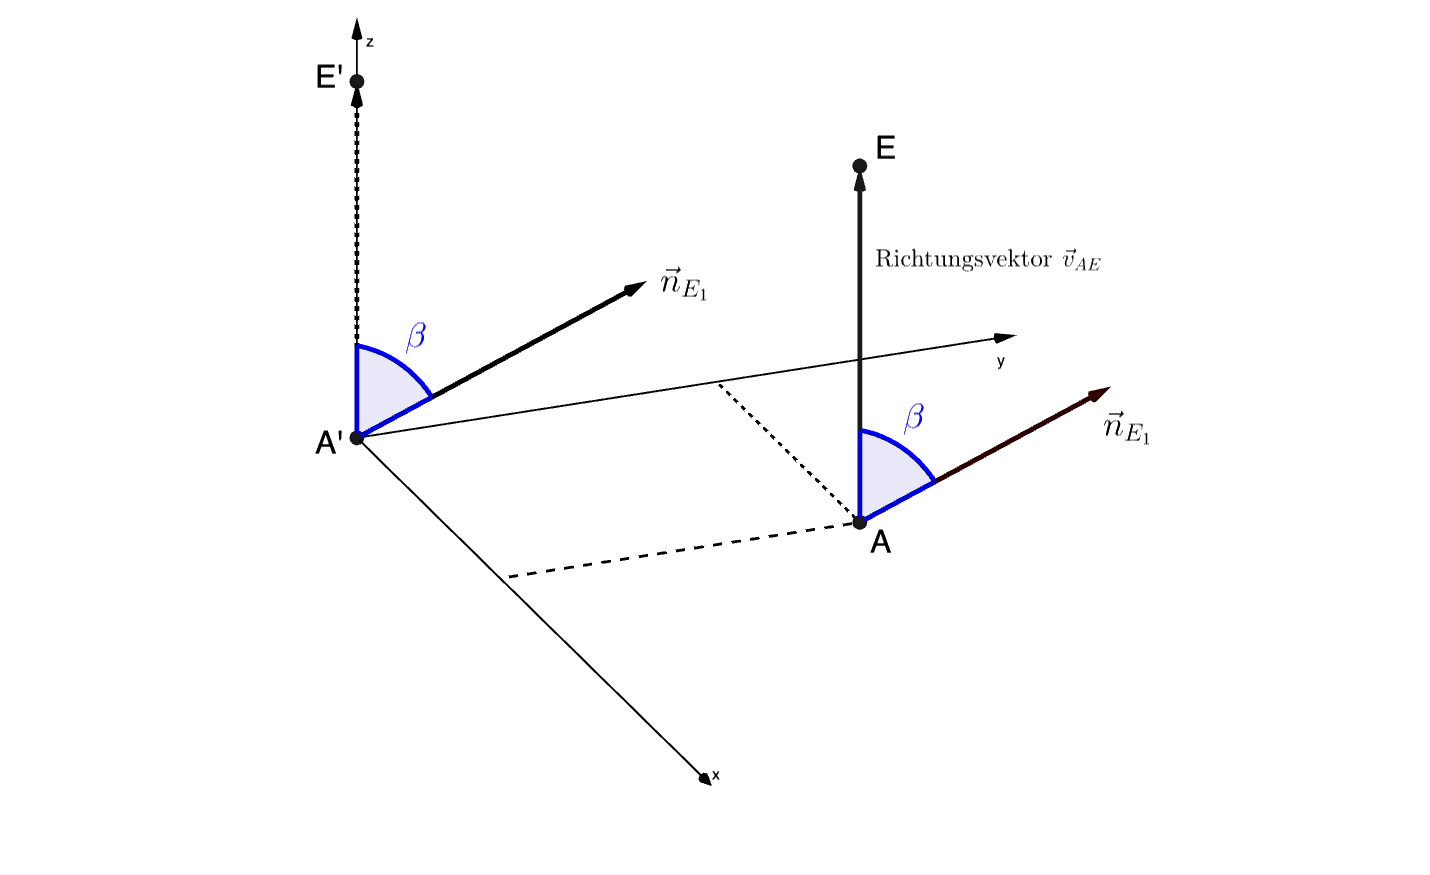
\includegraphics[width=10cm]{images/einleitung/VerschiebungKoordinatensystem.png}
        \caption{Beispiel der Translation des Richtungsvektors $\vec{v}_{AE}$. Der Winkel $\beta$ zum Normalenvektor $\vec{n}_{E_1}$ bleibt dabei erhalten.}
        \label{fig:beobachtungenOrthogonalprojektionWurfel}
    \end{figure}

Es lässt sich beobachten, dass die Strecken $\overline{CG}$, $\overline{CB}$ und $\overline{CD}$ den gleichen Winkel $\alpha$ mit dem Normalenvektor $\vec{n}_{E_1}$ einschliessen. Da alle Kanten des regulären Hexaeders zudem dieselbe Länge besitzen, sind auch ihre Projektionslängen identisch. Aus den vorangegangenen Überlegungen folgt, dass sämtliche Kanten des Würfels die gleiche Projektionslänge auf die Ebene $E_1$ aufweisen. Zur Berechnung dieser Länge können wir elementare trigonometrische Funktionen verwenden:

\begin{align} \label{eq:einführungsbeispielprojectionsimple}
    \|\Pi_{E_1}(\vec{v}_{CG})\| = \sin(\alpha) \cdot \|\vec{v}_{CG}\|,
\end{align}

wobei $\vec{v}_{CG}$ den Vektor der Kante $\overline{CG}$ repräsentiert und $\alpha$ der Winkel zwischen diesem Vektor und dem Normalenvektor $\vec{n}_{E_1}$ ist. Mit 
    \begin{align}
        \overline{CG}: \vec{v}_{CG}&=\begin{pmatrix} 0 \\ 0 \\ 1 \end{pmatrix},\|\vec{v}_{CG}\| = 1 \nonumber
    \end{align} sowie der Berechnungen
    \begin{align}
        \cos(\alpha) &= \frac{\vec{v}_{CG} \cdot \vec{n}_{E_1}}{\|\vec{v}_{CG}\| \|\vec{n}_{E_1}\|} = \frac{1}{\sqrt{3}} \nonumber \\
        \sin(\alpha) &= \sqrt{1-\cos^2(\alpha)} = \sqrt{\frac{2}{3}}, \nonumber
    \end{align}
    folgt aus Gleichung \eqref{eq:einführungsbeispielprojectionsimple}
    \begin{align}
        \|\Pi_{E_1}(\vec{v}_{CG})\| = \sqrt{\frac{2}{3}} \cdot 1= \sqrt{\frac{2}{3}} . \nonumber
    \end{align}
    Um die Summe aus Gleichung \eqref{eq:hypothese1} zu erhalten, müssen wir über alle Kanten in $K_W$ summieren und erhalten 
    \begin{align} \label{eq:summeebene1}
        \sum_{k \in K_W} \|\Pi_{E_1}(\vec{v}_{k})\| = 12 \cdot \sqrt{\frac{2}{3}} = 4\sqrt{6}.
    \end{align}
    
Wir behalten dieses Ergebnis im Hinterkopf und betrachten nun die Orthogonalprojektion auf die Ebene $E_2$ mit dem Einheitsnormalenvektor
    \begin{align}
        \vec{n}_{E_2} = \frac{1}{\sqrt{2}}\begin{pmatrix} 1 \\ -1 \\ 0 \end{pmatrix} .\nonumber
    \end{align}
    
    
    \begin{figure}[htp]
    \centering
    \includegraphics[width=0.7\textwidth, keepaspectratio]{images/einleitung/WürfelE2.png}
    \caption{Projektion der Kanten des Würfels auf die Ebene $E_2$ mit Normalenvektor $\vec{n}_{E_2}$.}
    \label{fig:würfelE2}
    \end{figure}
    
Aufgrund der Symmetrie des regulären Hexaeders können wir bei dieser Projektion zwei verschiedene Gruppen von Kanten unterscheiden:
\begin{itemize}
    \item Vier Kanten liegen parallel zur Ebene $E_2$ bzw. stehen orthogonal auf dem Normalenvektor $\vec{n}_{E_2}$, wie beispielsweise die Kante $\overline{CG}$.
    \item Die restlichen acht Kanten schliessen alle denselben Winkel $\alpha$, siehe Abbildung \ref{fig:würfelE2},mit dem Normalenvektor $\vec{n}_{E_2}$ ein, wie beispielsweise die Kante $\overline{GH}$.
\end{itemize}

Für die parallel zur Ebene $E_2$ verlaufenden Kanten gilt, dass ihre Länge bei der Projektion erhalten bleibt: 
\begin{align}
    \|\Pi_{E_2}(\vec{v}_{CG})\| = 1. \nonumber
\end{align}
    Für die anderen acht Kanten berechnen wir die Projektionslänge analog zu Gleichung \eqref{eq:einführungsbeispielprojectionsimple}. Da der Richtungsvektor $\vec{v}_{GH} = (1, 0, 0)^T$ einen Winkel von $\alpha = 45^\circ$ mit dem Normalenvektor $\vec{n}_{E_2}$ einschliesst, erhalten wir
\begin{align}
     \|\Pi_{E_2}(\vec{v}_{GH})\| = \sin\left(\frac{\pi}{4}\right) \cdot \|\vec{v}_{GH}\| = \frac{\sqrt{2}}{2} \cdot 1 = \frac{\sqrt{2}}{2}. \nonumber
\end{align}

Die Summation über alle 12 Kanten des regulären Hexaeders $W$ ergibt somit
\begin{align} \label{eq:summeebene2}
    \sum_{k \in K_W} \|\Pi_{E_2}(\vec{v}_k)\| = 4 \cdot 1 + 8 \cdot \frac{\sqrt{2}}{2} = 4 + 4\sqrt{2} = 4(1+\sqrt{2}).
\end{align}
Ein Vergleich der Ergebnisse aus den Gleichungen \eqref{eq:summeebene1} und \eqref{eq:summeebene2} zeigt deutlich, dass die Summen nicht übereinstimmen. Folglich ist die Summe der projizierten Kantenlängen unter einer Orthogonalprojektion nicht unabhängig von der Ebene. Die ursprüngliche Hypothese ist damit widerlegt. Dies beendet unser Beispiel.    
\end{example}


Wie wir in Beispiel \ref{ex:wuerfelprojektionen} gesehen haben, ist die Summe der projizierten Kantenlängen einer Orthogonalprojektion nicht unabhängig von der Projektionsebene. Eine invariante Eigenschaft unter Orthogonalprojektionen zu finden, scheint daher nicht trivial zu sein. Betrachten wir jedoch die Ergebnisse aus den Gleichungen \eqref{eq:summeebene1} und \eqref{eq:summeebene2} erneut, fällt bei genauerem Hinsehen auf, dass die Werte sehr nah beieinander liegen. Bei weiterer Untersuchung zeigt sich eine interessante Gesetzmässigkeit: Verwendet man die Quadrate der projizierten Kantenlängen scheinen die Summen tatsächlich identisch zu sein.

\begin{example} [Würfelprojektionen revisited] \label{ex:wuerfelprojektionen_revisited}
Wir passen unsere Hypothese an und betrachten die Summe der quadrierten Längen, d.h.
\begin{align}
    \sum_{k \in K_W} \|\Pi_{E_1}(\vec{v}_k)\|^2 = \sum_{k \in K_W} \|\Pi_{E_2}(\vec{v}_k)\|^2. \nonumber
\end{align}

Analog zu Beispiel \ref{ex:wuerfelprojektionen} berechnen wir die quadrierten Projektionslängen. Für die Ebene $E_1$ erhalten wir 
\begin{align}
    \sum_{k \in K_W} \|\Pi_{E_1}(\vec{v}_k)\|^2 = 12 \cdot \left(\sqrt{\frac{2}{3}}\right)^2 = 12 \cdot \frac{2}{3} = 8, \nonumber
\end{align}
und für die Ebene $E_2$
\begin{align}
    \sum_{k \in K_W} \|\Pi_{E_2}(\vec{v}_k)\|^2 = 4 \cdot 1^2 + 8 \cdot \left(\frac{\sqrt{2}}{2}\right)^2 = 4 + 8 \cdot \frac{1}{2} = 8. \nonumber
\end{align}
Dies bestätigt die angepasste Hypothese für diese beiden Fälle. Dies beendet unser Beispiel.
\end{example}

In Beispiel \ref{ex:wuerfelprojektionen_revisited} haben wir gesehen, dass unsere Vermutung für die Ebenen $E_1$ und $E_2$ zutrifft. Wie sich im Folgenden zeigen wird, ist dies kein Zufall. Diese Invarianz gilt nicht nur für das reguläre Hexaeder, sondern allgemein für alle Polyeder im $\mathbb{R}^3$, die gewisse Symmetriebedingungen erfüllen.

\subsubsection{Aufgaben}
\begin{exercise} \label{ex:verificationeinstiegesbeispielEbene3}
    Verifizieren Sie das Resultat aus Beispiel \ref{ex:wuerfelprojektionen_revisited} für die Ebene 
    \begin{align}
        E_3:\ x = 0. \nonumber
    \end{align}
    Berechnen Sie hierzu die Summe der quadrierten Längen der orthogonal projizierten Kanten des regulären Hexaeders mit Kantenlänge $1$ auf $E_3$.
\end{exercise}

\begin{exercise} \label{ex:geradesprisma}
    Betrachten Sie ein gerades Prisma mit einer quadratischen Grundfläche der Seitenlänge $a$ und der Höhe $h$, wobei $a \neq h$. Geben Sie zwei Projektionsebenen an und zeigen Sie durch Berechnung der jeweiligen Orthogonalprojektionen, dass die in Beispiel \ref{ex:wuerfelprojektionen_revisited} beschriebene Invarianz der quadrierten Kantenlängensumme für diesen Körper im Allgemeinen nicht gilt.
\end{exercise}
\newpage
%\subsection{Didaktische Überlegungen}
\subsection{Reguläre Polyeder}
In dieser Arbeit werden wir uns intensiv mit den Symmetrieeigenschaften von drei spezifischen regulären Polyedern auseinandersetzen: dem regulären \textit{Tetraeder}, dem regulären \textit{Hexaeder} und dem regulären \textit{Ikosaeder}. Bevor wir jedoch im Detail auf diese Körper eingehen, geben wir eine kurze Einführung in die Geschichte der \textit{regulären Polyeder}. Dieser Abschnitt basiert auf den Ausführungen von P.R. Cromwell \cite[Kap.~2]{cromwell_polyhedra_1997} und H.S.M. Coxeter \cite[Kap.~1.2-1.3,~2.1]{coxeter_regular_polytopes_1973}.

\subsubsection{Historische Entwicklung}
Die Beschäftigung mit regulären Polyedern gehört zu den ältesten Themen der Geometrie. Ein Polyeder (griechisch für „Vielflächner“) ist ein dreidimensionaler Körper, der ausschliesslich von ebenen Flächen begrenzt wird. Unter diesen nehmen die regulären Polyeder eine Sonderstellung ein, da sie ein Höchstmass an Gleichmässigkeit und Symmetrie aufweisen. Bereits in der griechischen Antike faszinierten diese Formen Mathematiker und Philosophen gleichermassen. Peter Cromwell beschreibt in seinem Werk \textit{Polyhedra}, wie diese Körper im 13. Buch von Euklids „Elementen“ erstmals systematisch erfasst wurden. Euklid lieferte dort den entscheidenden Beweis, dass es im dreidimensionalen Raum genau fünf dieser perfekten Formen gibt – die sogenannten Platonischen Körper. Während sie in der Antike oft als Symbole für die Naturelemente dienten, siehe Abbildung \ref{fig:platonicsolids}, betrachten wir sie heute primär als Untersuchungsobjekte der Gruppentheorie und Symmetrielehre. H.S.M. Coxeter, einer der bedeutendsten Geometer des 20. Jahrhunderts, legte mit seinem Buch \textit{Regular Polytopes} das Fundament dafür, diese Körper nicht nur als starre Objekte, sondern als Resultat von Spiegelungen und Drehungen zu verstehen.

\begin{figure}[htp]
\centering
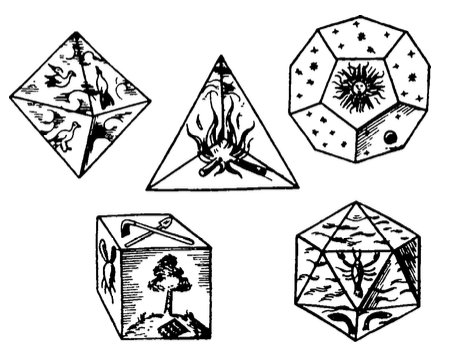
\includegraphics[width=10cm]{images/polyeder/platonic_solids.png}
\caption{Zeichnung der Platonischen Körper von Johannes Kepler aus \cite{cromwell_polyhedra_1997}. Obere Reihe (v.l.n.r.): \textit{Oktaeder}, \textit{Tetraeder}, \textit{Dodekaeder}. Untere Reihe (v.l.n.r.): \textit{Hexaeder}, \textit{Ikosaeder}.}
\label{fig:platonicsolids}
\end{figure}

\subsubsection{Polyeder}
Bevor wir die Besonderheiten der Symmetrie untersuchen, müssen wir klären, was genau ein Polyeder im mathematischen Sinne definiert. Ein Polyeder (von griechisch \textit{poly} für „viel“ und \textit{hedra} für „Sitz“ oder „Fläche“) ist ein dreidimensionaler Körper, dessen Oberfläche aus ebenen Polygonen (Vielecken) besteht. Nach Cromwell lässt sich ein Polyeder als eine Ansammlung von Flächen beschreiben, die so miteinander verbunden sind, dass sie einen abgeschlossenen Raumteil umschliessen. Dabei müssen zwei wesentliche Bedingungen erfüllt sein:

\begin{itemize}
    \item Jede Kante gehört zu genau zwei Flächen.
    \item Der Körper ist zusammenhängend: Man kann von jeder Fläche zu jeder anderen gelangen, indem man über die Kanten wandert.
\end{itemize}

Die Schnittpunkte, an denen mindestens drei Flächen (und damit mindestens drei Kanten) aufeinandertreffen, bezeichnen wir als Ecken. Ein Tetraeder besitzt beispielsweise 6 Kanten und 4 Ecken (siehe Abbildung \ref{fig:tetraeder}).

\begin{figure}[htp]
\centering
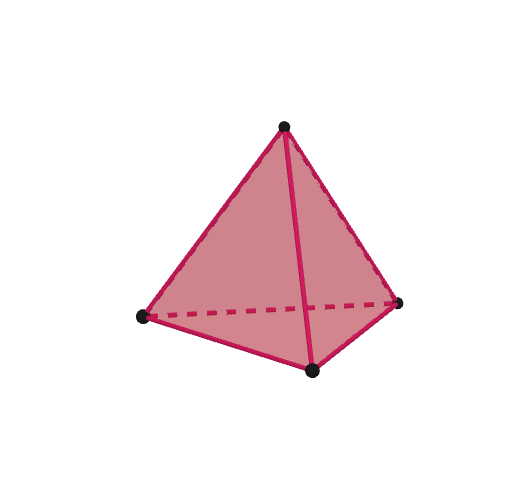
\includegraphics[width=0.4\textwidth]{images/polyeder/tetraeder.png}
\caption{Reguläres Tetraeder.}
\label{fig:tetraeder}
\end{figure}



Alltagsbeispiele für Polyeder sind etwa Pakete oder würfelförmige Regale. Sobald jedoch gekrümmte Begrenzungsflächen vorhanden sind – wie bei einer Kugel oder einer Getränkedose –, handelt es sich nicht mehr um ein Polyeder (siehe Abbildung \ref{fig:auswahl_polyeder}).

\begin{figure}[htbp]
     \centering
     \begin{subfigure}[b]{0.3\textwidth}
         \centering
         \includegraphics[width=\textwidth]{images/polyeder/kuppelhaus_düsseldorf.jpg}
         \caption{Kuppelhaus des botanischen Gartens in Düsseldorf.}
         \label{fig:kuppelhaus_düsseldorf}
     \end{subfigure}
     \hfill
     \begin{subfigure}[b]{0.3\textwidth}
         \centering
         
\includegraphics[width=\textwidth]{images/polyeder/kallax_ikea.png}
         \caption{Regalsystem.}
         \label{fig:kallaxikea}
     \end{subfigure}
     \hfill
     \begin{subfigure}[b]{0.3\textwidth}
         \centering
         
\includegraphics[width=\textwidth]{images/polyeder/paket.png}
         \caption{Quaderförmiges Paket.}
         \label{fig:Paket}
     \end{subfigure}
        \caption{Beispiele für Polyeder im Alltag und in der Architektur.}
        \label{fig:auswahl_polyeder}
\end{figure}

Damit ein Polyeder als \textit{regulär} eingestuft wird, müssen laut Coxeter zwei strenge Anforderungen an seine Regelmässigkeit erfüllt sein:

\begin{itemize}
    \item \textbf{Flächenregularität}: Alle Seitenflächen sind kongruente, reguläre Vielecke. Dies bedeutet, dass alle Kanten gleich lang und alle Innenwinkel der Flächen identisch sind.
    \item \textbf{Eckenregularität}: An jeder Ecke des Polyeders treffen stets gleich viele Flächen in der immer gleichen Anordnung zusammen.
\end{itemize}

Diese Struktur wird mathematisch durch das Schläfli-Symbol $\{p, q\}$ zusammengefasst. Dabei steht $p$ für die Anzahl der Ecken einer einzelnen Fläche und $q$ für die Anzahl der Flächen, die an einer Ecke zusammentreffen. Ein Würfel besteht aus Quadraten ($p=4$), von denen drei an jeder Ecke zusammenkommen ($q=3$), was zum Symbol $\{4, 3\}$ führt. 

Von diesen regulären Polyedern, auch als Platonische Körper bekannt, existieren exakt fünf:
\begin{itemize}
    \item \textbf{Reguläres Tetraeder}: (griech. \textit{tetra} = vier) Begrenzt von vier regulären Dreiecken.
    \item \textbf{Reguläres Hexaeder}: (griech. \textit{hex} = sechs) Der Würfel, begrenzt von sechs Quadraten.
    \item \textbf{Reguläres Oktaeder}: (griech. \textit{oktō} = acht) Begrenzt von acht regulären Dreiecken.
    \item \textbf{Reguläres Dodekaeder}: (griech. \textit{dōdeka} = zwölf) Begrenzt von zwölf regulären Fünfecken.
    \item \textbf{Reguläres Ikosaeder}: (griech. \textit{eíkosi} = zwanzig) Begrenzt von zwanzig regulären Dreiecken.
\end{itemize}



Es existieren verschiedene Beweise dafür, dass es genau fünf reguläre Polyeder gibt. Ein geometrischer Beweis von Euklid basiert auf den Innenwinkeln der Flächen. Ein weiterer, algebraischer Beweis stammt von Leonhard Euler; dieser nutzt den Polyedersatz und benötigt keine Betrachtung der Winkel. Da diese Beweise für den weiteren Verlauf dieser Arbeit nicht unmittelbar relevant sind, verweisen wir auf die entsprechende Literatur \cite[Kap.~2]{coxeter_regular_polytopes_1973, cromwell_polyhedra_1997}. Im nächsten Abschnitt werden wir uns intensiv mit den Symmetriegruppen dieser Körper beschäftigen.


\subsubsection{Aufgaben}

\begin{exercise} \label{ex:polyederalltag}
    Nennen Sie drei weitere Beispiele für Polyeder aus Ihrem Alltag, die noch nicht im Text erwähnt wurden. Begründen Sie kurz anhand der Definition, warum es sich um Polyeder handelt.
\end{exercise}

\begin{exercise} \label{ex:polyederbeispiele}
    Prüfen Sie anhand der Definition eines Polyeders, ob es sich bei den folgenden Objekten um ein solches handelt:
    \begin{itemize}
        \item[a)] der \textit{Adidas Fevernova} (offizieller Fussball der WM 2002),
        \item[b)] ein klassischer Spielwürfel mit abgerundeten Ecken.
    \end{itemize}
    Begründen Sie Ihre Antwort. Handelt es sich zudem um \textbf{reguläre} Polyeder?
\end{exercise}
\newpage
\subsection{Symmetriegruppen} \label{sec:symmetrieeigenschaftwürfel}

Wir definieren die Symmetriegruppe von einem Polyeder wie folgt
\begin{definition}
Sei $X \subset \mathbb{R}^n$ eine geometrische Figur (in unserem Fall ein Polyeder im $\mathbb{R}^3$). Eine Symmetrie von $X$ ist eine abstandserhaltende Abbildung (Isometrie) $f: \mathbb{R}^n \to \mathbb{R}^n$, die die Figur als Ganzes auf sich selbst abbildet, für die also gilt: $f(X) = X$. Die Symmetriegruppe $S(X)$ ist die Menge all dieser Symmetrien von $X$. Die Gruppenoperation ist dabei die einfache Hintereinanderausführung (Komposition) der Abbildungen.
\end{definition}

\begin{example}[Symmetriegruppe: Reguläres Tetraeder] \label{ex:regulaeres_tetraeder}
Das reguläre Tetraeder hat genau 12 Kongruenzabbildungen. Diese kann man auf mehrere Arten finden. Einerseits wissen wir, dass ein Tetraeder 6 Kanten besitzt, welche in 2 Richtungen orientiert werden können. Daraus folgt, dass es $12$ Abbildungen gibt. Andererseits können wir die Abbildungen auch zählen. 
\begin{center}
\begin{tabular}{ |c|c|c|c| } 
 \hline
 Beschreibung & Symmetrieachse & Periodizität & Anzahl Abbildungen \\ 
 \hline
 Identität & - & - & 1 \\ 
 Ecke, Mitte geg. Dreiecksfläche& K-M & $\frac{\pi}{3}$ & $2*4 = 8$  \\ 
 Kante, Kante& K-K & $\frac{\pi}{2}$ & $1*3=3$  \\ 
 \hline
  & & & 12 \\ 
 \hline
\end{tabular}
\end{center}
\end{example}

\begin{example}[Reguläres Hexaeder] \label{ex:regulaeres_hexaeder}
TODO:...
\end{example}

\begin{example}[Reguläres Ikosaeder] \label{ex:regulaeres_ikosaeder}
TODO:...
\end{example}


\subsubsection{Richtungserhaltende Abbildungen}
\begin{align}
    todo:
\end{align}


\subsubsection{Irreduzibilität}
In diesem Abschnitt untersuchen wir eine grundlegende Eigenschaft der orientierungserhaltenden Symmetriegruppen des regulären Tetraeders, Hexaeders und Ikosaeders. Wir bezeichnen mit $T$ die Gruppe der orientierungserhaltenden Symmetrien (Drehgruppe) des Tetraeders sowie analog mit $H$ und $I$ jene des Hexaeders respektive des Ikosaeders.

\begin{definition}
Sei $V$ ein Vektorraum (in unserem Fall der $\mathbb{R}^3$) und $G$ eine Gruppe von linearen Abbildungen, die auf $V$ operiert. Ein Unterraum $U \subseteq V$ heißt $G$-invariant (oder stabil unter $G$), wenn für jedes Element $g \in G$ und jeden Vektor $u \in U$ gilt, dass das Bild $g(u)$ wieder in $U$ liegt. Die Operation der Gruppe $G$ auf dem Raum $V$ heißt irreduzibel, wenn die einzigen $G$-invarianten Unterräume der triviale Nullraum $\{0\}$ und der gesamte Raum $V$ selbst sind. Gibt es hingegen einen echten invarianten Unterraum (also $U \neq \{0\}$ und $U \neq V$), so nennt man die Gruppe reduzibel.
\end{definition}


\begin{lemma} \label{lemma:irreduzibelsymmetriegruppen}
    Die orientierungserhaltenden Symmetriegruppen des Tetraeders ($T$), Hexaeders ($H$) und Ikosaeders ($I$) operieren irreduzibel auf dem $\mathbb{R}^3$. Das bedeutet, dass unter der Wirkung dieser Gruppen keine nicht-trivialen invarianten Unterräume existieren.
\end{lemma}

\begin{proof}
    Angenommen, eine Gruppe $\Omega \in \{T, H, I\}$ operiere reduzibel auf dem $\mathbb{R}^3$. Dann existiert per Definition ein echter invarianter Unterraum $U \subset \mathbb{R}^3$ der Dimension 1 (eine Gerade durch den Ursprung) oder der Dimension 2 (eine Ebene durch den Ursprung). Invariant bedeutet, dass für jedes $R \in \Omega$ und jeden Vektor $\vec{u} \in U$ auch das Bild $R\vec{u}$ wieder in $U$ liegt.

    Wir zeigen zunächst, dass in beiden Fällen eine invariante Gerade $g$ existieren muss:
    \begin{itemize}
        \item Falls $\dim(U) = 1$, ist $U$ selbst die invariante Gerade $g$.
        \item Falls $\dim(U) = 2$, muss der Normalenvektor $\vec{n}_U$ der Ebene $U$ invariant unter allen Drehungen $R \in \Omega$ sein (bis auf das Vorzeichen), da die Drehung einer Ebene deren Normale festlässt oder spiegelt. Somit bildet die durch $\vec{n}_U$ aufgespannte Gerade die gesuchte invariante Gerade $g$.
    \end{itemize}

    Sei $\vec{v}_g$ ein Richtungsvektor der Geraden $g$. Da $g$ invariant unter allen Drehungen $R \in \Omega$ ist, gibt es für das Bild $R\vec{v}_g$ nur zwei Möglichkeiten:
    \begin{itemize}
        \item $R\vec{v}_g = \vec{v}_g$ (der Vektor bleibt fix), oder
        \item $R\vec{v}_g = -\vec{v}_g$ (der Vektor wird um $180^\circ$ gedreht).
    \end{itemize}

    Nun enthalten alle betrachteten Gruppen $\{T, H, I\}$ jedoch Drehungen um $120^\circ$ (entsprechend der Symmetrie der Flächen oder Ecken). Eine $120^\circ$-Drehung kann einen Vektor nur dann auf $\vec{v}_g$ oder $-\vec{v}_g$ abbilden, wenn $\vec{v}_g$ selbst auf der Drehachse liegt. Damit die Gerade $g$ für die \textit{gesamte} Gruppe invariant ist, müsste sie also die gemeinsame Drehachse \textit{aller} $120^\circ$-Drehungen der Gruppe sein.

    Wir wissen jedoch:
    \begin{itemize}
        \item Das Tetraeder besitzt 4 solcher Drehachsen (durch die Ecken),
        \item das Hexaeder besitzt ebenfalls 4 (die Raumdiagonalen),
        \item das Ikosaeder besitzt 10 solcher Drehachsen (durch die gegenüberliegenden Ecken).
    \begin{figure}[htp]
        \centering
        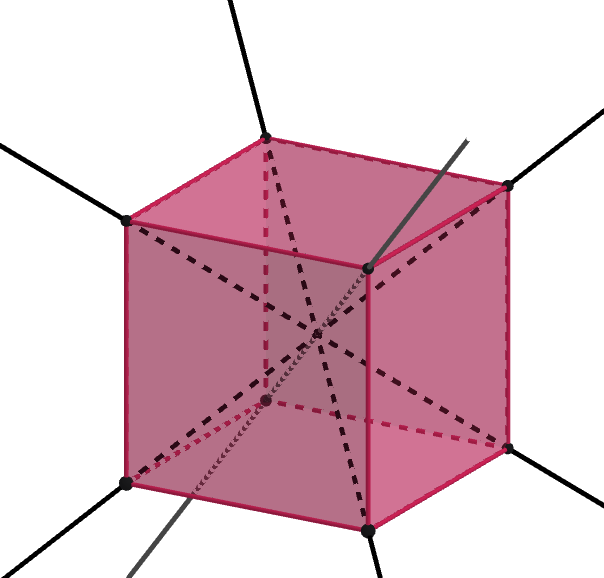
\includegraphics[width=0.6\textwidth]{images/polyeder/raumdiagonalen.png}
        \caption{Drehachsen eines regulären Hexaeders durch gegenüberliegende Ecken ($120^\circ$-Drehungen).}
        \label{fig:drehachsen}
    \end{figure}
    \end{itemize}
    Da diese Achsen nicht identisch sind, kann keine einzelne Gerade unter allen Elementen von $\Omega$ invariant sein. Dies führt zu einem Widerspruch, womit die Irreduzibilität bewiesen ist.
\end{proof}


\subsubsection{Orthogonale Matrizen} \label{sec:orthogonalrotation}
In diesem Abschnitt zeigen wir, dass Matrizen, die eine Drehung im euklidischen Raum beschreiben, stets orthogonale Matrizen sind.

\begin{lemma} \label{lemma:drehungensindorthogonalmatrizen}
    Eine Matrix $R \in \mathbb{R}^{n \times n}$, die eine Drehung repräsentiert, ist eine orthogonale Matrix. Es gilt somit $R^T R = I$, wobei $I$ die Einheitsmatrix bezeichnet.
\end{lemma}

\begin{proof}
    Seien $\vec{v}, \vec{w} \in \mathbb{R}^n$. Eine Drehung ist eine Isometrie; per Definition bleiben unter dieser Transformation zwei Eigenschaften invariant:
\begin{itemize}
    \item Die Längen der Vektoren verändern sich nicht ($\|\vec{v}\| = \|R\vec{v}\|$).
    \item Der Winkel zwischen zwei Vektoren bleibt erhalten.
\end{itemize}
Da eine Drehung somit das Skalarprodukt (und damit Längen und Winkel) erhält, muss für beliebige Vektoren $\vec{v}$ und $\vec{w}$ gelten
\begin{align*}
    (R\vec{v}) \cdot (R\vec{w}) = \vec{v} \cdot \vec{w}.
\end{align*}
Unter Verwendung der Matrixschreibweise für das Skalarprodukt $(\vec{a} \cdot \vec{b} = \vec{a}^T \vec{b})$ erhalten wir:
\begin{alignat*}{2}
    & (R\vec{v})^T (R\vec{w}) &&= \vec{v}^T\vec{w} \\
    \iff & \vec{v}^T R^T R \vec{w} &&= \vec{v}^T\vec{w} \\
    \iff & \vec{v}^T (R^T R) \vec{w} &&= \vec{v}^T I \vec{w}.
\end{alignat*}
Da diese Gleichung für alle Vektoren $\vec{v}, \vec{w} \in \mathbb{R}^n$ erfüllt sein muss, folgt daraus unmittelbar die Matrizengleichung:
\begin{align}
    R^T R = I. \nonumber
\end{align}
\end{proof}


\newpage

\subsection{Orthogonalprojektion auf eine Ebene im \texorpdfstring{$\mathbb{R}^3$}{R³}}

In diesem Text arbeiten wir primär mit Projektionen im dreidimensionalen euklidischen Raum.

\begin{definition} \label{def:orthogonalprojektion}
Sei $E \subset \mathbb{R}^3$ eine Ebene durch den Ursprung mit dem Einheitsnormalenvektor $\vec{n}$. Die Orthogonalprojektion $\Pi_E: \mathbb{R}^3 \rightarrow E$ ist eine lineare Abbildung, die jedem Vektor $\vec{v} \in \mathbb{R}^3$ seinen Bildpunkt in $E$ so zuordnet, dass der Differenzvektor $\vec{v} - \Pi_E(\vec{v})$ parallel zu $\vec{n}$ steht.
\end{definition}

Für die Beweise in Kapitel \ref{sec:orthogonalprojektionen} werden wir explizite Orthogonalprojektionen berechnen. Zur Vorbereitung leiten wir hier die allgemeine Abbildungsvorschrift her. Jeder Vektor $\vec{v}$ lässt sich eindeutig in zwei Komponenten zerlegen:
\begin{align} \label{eq:vektor_parallel_senkrecht}
    \vec{v} = \vec{v}_{\parallel} + \vec{v}_{\perp},
\end{align}
wobei gilt:
\begin{itemize}
    \item $\vec{v}_{\parallel}$ liegt in der Ebene $E$ (die projizierte Komponente),
    \item $\vec{v}_{\perp}$ steht senkrecht auf der Ebene $E$ und ist somit parallel zum Einheitsnormalenvektor $\vec{n}$.
\end{itemize}

Da $\vec{v}_{\perp}$ parallel zu $\vec{n}$ ist, existiert ein Skalar $\alpha \in \mathbb{R}$ mit $\vec{v}_{\perp} = \alpha \vec{n}$. Um $\alpha$ zu bestimmen, bilden wir das Skalarprodukt mit $\vec{n}$:
\begin{align} \label{eq:skalar_senkrecht}
    \vec{n} \cdot \vec{v} &= \vec{n} \cdot (\vec{v}_{\parallel} + \vec{v}_{\perp}) \nonumber \\
    &= \vec{n} \cdot \vec{v}_{\parallel} + \vec{n} \cdot (\alpha \vec{n}) \nonumber \\
    &= 0 + \alpha (\vec{n} \cdot \vec{n}) = \alpha,
\end{align}
wobei wir $\vec{n} \cdot \vec{v}_{\parallel} = 0$ (da $\vec{v}_{\parallel} \in E$) und $\vec{n} \cdot \vec{n} = 1$ (da $\|\vec{n}\|=1$) genutzt haben. Einsetzen in \eqref{eq:vektor_parallel_senkrecht} liefert:

\begin{align} \label{eq:projectionwithvectorandnormal}
    \Pi_{E}(\vec{v}) &= \vec{v}_{\parallel} = \vec{v} - \vec{v}_{\perp} \nonumber \\
    &= \vec{v} - \alpha \vec{n} \nonumber \\
    &= \vec{v} - (\vec{n} \cdot \vec{v}) \vec{n}.
\end{align}



In Matrixschreibweise lässt sich das Skalarprodukt $(\vec{n} \cdot \vec{v})\vec{n}$ als dyadisches Produkt $\vec{n}\vec{n}^T \vec{v}$ ausdrücken. Damit erhalten wir die Projektionsmatrix:

\begin{align} \label{eq:ortho_proj_matrix_notation}
    \Pi_{E}(\vec{v}) &= \vec{v} - (\vec{n}\vec{n}^T) \vec{v} \nonumber \\
    &= (I - \vec{n}\vec{n}^T) \vec{v}.
\end{align}

\subsubsection{Aufgaben}
\begin{exercise} \label{ex:verifizierungwuerfelprojektion}
Verifizieren Sie die Resultate für die Ebenen $E_1$ und $E_2$ aus Beispiel \ref{ex:wuerfelprojektionen} mithilfe der Matrixdarstellung aus Gleichung \eqref{eq:ortho_proj_matrix_notation}.
\end{exercise}

